\documentclass{article}

% if you need to pass options to natbib, use, e.g.:
%     \PassOptionsToPackage{numbers, compress}{natbib}
% before loading neurips_2018

% ready for submission
% \usepackage{neurips_2018}

% to compile a preprint version, e.g., for submission to arXiv, add add the
% [preprint] option:
 % \usepackage[preprint]{neurips_2018}

% to compile a camera-ready version, add the [final] option, e.g.:
 \usepackage[nonatbib]{neurips_2019}
% to avoid loading the natbib package, add option nonatbib:
 % \usepackage[nonatbib]{neurips_2019}
\usepackage{graphicx}
\usepackage[utf8]{inputenc} % allow utf-8 input
\usepackage[T1]{fontenc}    % use 8-bit T1 fonts
\usepackage{hyperref}       % hyperlinks
\usepackage{url}            % simple URL typesetting
\usepackage{booktabs}       % professional-quality tables
\usepackage{amsfonts}       % blackboard math symbols
\usepackage{nicefrac}       % compact symbols for 1/2, etc.
\usepackage{microtype}      % microtypography
\usepackage{amsmath}
\usepackage{bm}
\usepackage{subfig}
\usepackage[english]{babel}
\usepackage{algorithm}
\usepackage{algorithmic}
\usepackage{appendix}
\newtheorem{theorem}{Theorem}
\newtheorem{lemma}{Lemma}
\newtheorem{prop}{Proposition}
\newtheorem{ass}{Assumption}
\newtheorem{defn}{Definition}
\newtheorem{exam}{Example}
\newtheorem{proof}{Proof}
\input macros.tex
\usepackage{dsfont}


\newcommand*{\KeepStyleUnderBrace}[1]{%f
  \mathop{%
    \mathchoice
    {\underbrace{\displaystyle#1}}%
    {\underbrace{\textstyle#1}}%
    {\underbrace{\scriptstyle#1}}%
    {\underbrace{\scriptscriptstyle#1}}%
  }\limits
}

\usepackage{xr}
\externaldocument{nips_2019_supp}


\title{Multi-way block localization vis sparse tensor clustering}


\author{%
Yuchen Zeng \\
 University of Wisconsin -- Madison\\
 \texttt{yzeng58@wisc.edu} \\
\And
Miaoyan Wang \\
 University of Wisconsin -- Madison\\
\texttt{miaoyan.wang@wisc.edu} \\
}

\begin{document}

\maketitle

\begin{abstract}
We consider the task of simultaneously clustering each mode of a large noisy tensor. We assume that the tensor elements are distributed with a block-specific mean and propose a least-square estimation for multi-way clustering. An $\ell_1$ penalty is applied to the block-means in order to select and identify important blocks. We show that our method is applicable to large tensors with a wide range of multi-way cluster structure, including a single block, multiple blocks, checkerboard clusters, 1-way or lower-way blocks. Our proposal amounts to a sparse, multi-way version of $k$-mean clustering, and a relaxation of our proposal yields the tensor Tucker decomposition. The performance of our proposals are demonstrated in simulations and on... 
\end{abstract}

\section{Introduction}
In recent years, much interest has centered around the unsupervised analysis of high-dimensional high-order tensor data. 

Here is an example of tensor clustering by using our proposed method.
\begin{figure}[!h]
	\centering
	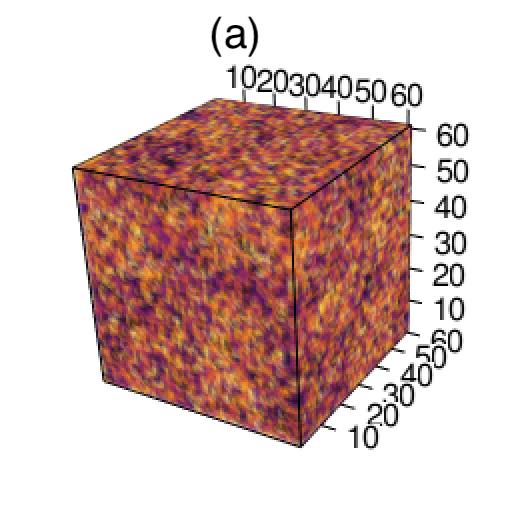
\includegraphics[scale=0.35]{figures/figure1/input.png}
	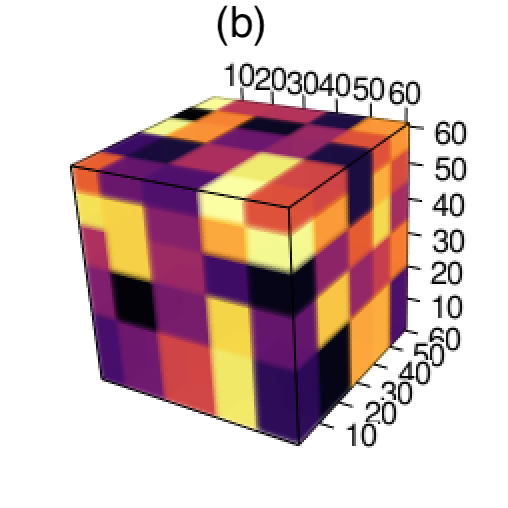
\includegraphics[scale=0.35]{figures/figure1/truth.png}
	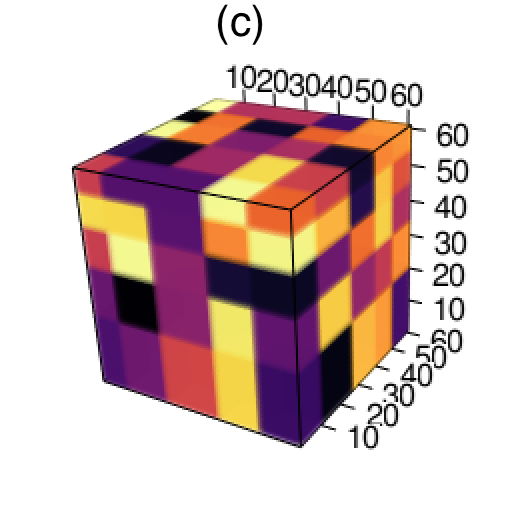
\includegraphics[scale=0.35]{figures/figure1/output.png}
	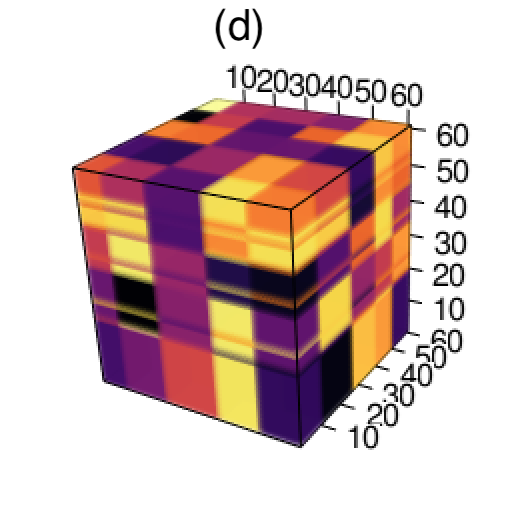
\includegraphics[scale=0.35]{figures/figure1/k_means.png}
	\caption{(a): a $60\times 60\times 60$ tensor with 5 clusters in each mode; (b): true underlying mean signal within each cluster; (c): mean signal estimated by our proposed approach with true number of clusters (5, 5, 5); (d): mean signal estimated by k-means clustering on each mode with true number of clusters (5 , 5, 5).}
	\label{fig:1}
\end{figure}

\begin{figure}
	\centering
	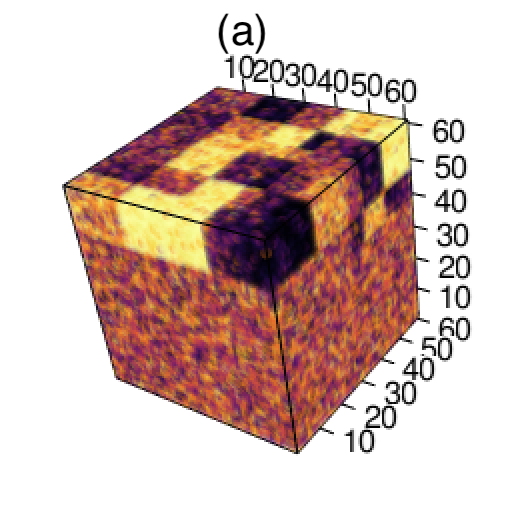
\includegraphics[scale=0.5]{figures/figure2/input.png}
	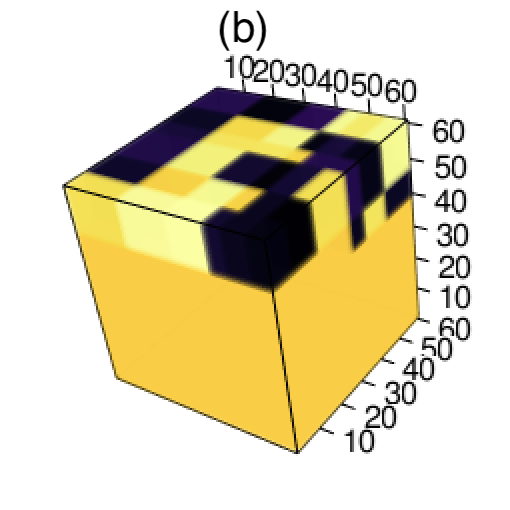
\includegraphics[scale=0.5]{figures/figure2/truth.png}
	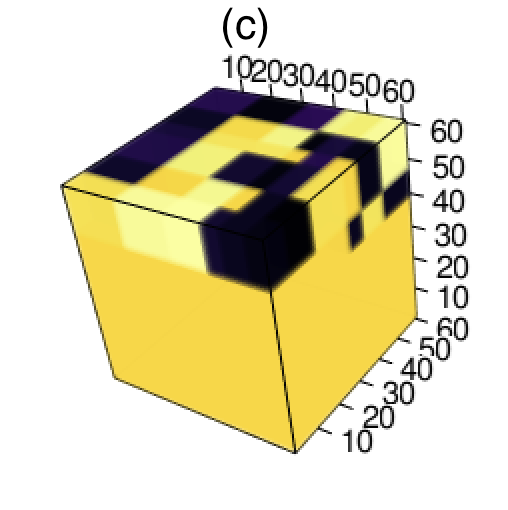
\includegraphics[scale=0.5]{figures/figure2/output.png}
	\caption{(a): $60\times 60\times 60$ sparse tensor; (b) true underlying means; (c) mean signal estimated by our approach with estimated number of clusters and estimated $\lambda$.}
	\label{fig2}
\end{figure}


\section{Preliminaries}

We say that an event $A$ occurs ``with high probability'' if $\mathbb{P}(\mA)$ tends to 1 as the dimension $d_{\min}=\min\{d_1,\ldots,d_k\}$ tends to infinity. We say that $A$ occurs ``with very high probability'' if $\mathbb{P}(A)$ tends to 1 faster than any polynomial of $d$. 


We use lower-case letters ($a,b,u,v,\ldots$) for scalars and vectors. We use upper-case boldface letters ($\mA,\mB,\mC,\ldots$) for matrices, and calligraphy letter ($\tA, \tB, \tC,\ldots$) for tensors of order $K\geq 3$. $\mx\otimes \my$ is the Kronecker product of two vectors. For any set $J$, $|J|$ denotes its cardinality. $[d]$ represents the set $\{1,2,\ldots,d\}$. 

A clustering of $d$ objects can be represented by a partition of the index set $[d]=\{1,\ldots,d\}$ into $R$ disjoint non-empty subsets. We refer to $R$ the clustering size. It is often convenient to represent the clustering (or partition) using the ``membership matrix''. A membership matrix $\mM$ is an $d$-by-$R$ matrix whose $(i,j)$-entry is 1 if and only if the element $i$ belongs to the cluster $j$, and 0 otherwise. Based on the definition, $\mM$ is binary matrix with orthogonal columns, and the matrix elements sum up to $d$. Throughout the paper, we will use the terms ``partition'', ``clustering'', and ``membership matrix'' exchangeably. 

For a higher-order tensor, the above concepts can be applied to each of the modes. We use the term ``mode-$k$ clustering'' to refer to the partition along the $k$-th mode of the tensor, and reserve ``block'' to mean a multi-way block in the Cartesian product of mode-$k$ clusters. 

\section{Tensor block model}
Let $\tY=\entry{y_{i_1,\ldots,i_K}}\in\mathbb{R}^{d_1\times \cdots\times d_K}$ denote an order-$K$, $(d_1,\ldots,d_K)$-dimensional data tensor. The main assumption on tensor block model is that the observed data tensor $\tY$ is a noisy realization of an underlying tensor that exhibits a checkerbox structure (see Figure~\ref{fig:1}). Specifically, suppose that there are $R_k$ clusters along the $k$-th mode of the tensor for $k\in[K]$. If the tensor entry $y_{i_1,\ldots,i_K}$ belongs to the block jointly determined by the $r_k$-th mode-$k$ cluster with $r_k\in[R_k]$, then we assume that 
\begin{equation}\label{eq:model}
y_{i_1,\ldots,i_K}=c_{r_1,\ldots,r_K}+\varepsilon_{i_1,\ldots,i_K},\quad \text{for }(i_1,\ldots,i_K)\in[d_1]\times\cdots\times [d_K],
\end{equation}
where $\mu_{r_1,\ldots,r_K}$ is the mean of the tensor block indexed by $(r_1,\ldots,r_K)$, and $\varepsilon_{i_1,\ldots,i_K}$'s are independent, mean-zero noise terms to be specified later. Our goal is to (i) find partitions along each of the modes, and (ii) estimate the block means $\{c_{r_1,\ldots,r_K}\}$, such that a corresponding blockwise-constant checkerbox structure emerges in the data tensor. 

The above tensor block model~\eqref{eq:model} falls into a larger class of non-overlapping, constant-mean clustering models~\cite{madeira2004biclustering}, in that each tensor entry belongs to exactly one block with a common mean. The model~\eqref{eq:model} can be equivalently expressed as a special tensor Tucker model,
\begin{equation}\label{eq:Tucker}
\tY=\tC\times_1\mM_1\times_2\cdots \times_K \mM_K+\tE,
\end{equation}
where $\tC\in\mathbb{R}^{R_1\times\cdots\times R_K}$ is a core tensor consisting of block means, $\mM_k \in\{0,1\}^{R_k\times d_k}$ are membership matrices indicating the block allocations along mode $k$ for $k\in[K]$, and $\tE=\entry{\varepsilon_{i_1,\ldots,i_K}}$ is the noise tensor. The distinction between our model~\eqref{eq:Tucker} and a classical Tucker model is that we require the factors $\mM_k$ to be membership matrices. Our model~\eqref{eq:Tucker} can be viewed as a super-sparse Tucker model, in the sense that the each column of $\mM_k$ consists of one copy of 1's and massive 0's. 

We now introduce the assumptions on the noise tensor $\tE$. We assume that $\varepsilon_{i_1,\ldots,i_K}$'s are independent, mean-zero, $\sigma$-subgaussian noises, where $\sigma>0$ is the subgaussianity parameter. More precisely, 
\begin{equation}\label{eq:noise}
\mathbb{E}e^{\lambda \varepsilon_{i_1,\ldots,i_K}}\leq e^{\lambda^2\sigma^2/2},\quad \text{for all } (i_1,\ldots,i_K)\in[d_1]\times\cdots\times[d_K] \ \text{and}\ \lambda\in\mathbb{R}.
\end{equation}
Th assumption~\eqref{eq:noise} is fairly general, which includes many common noises, such as Gaussian errors, Bernoulli errors, bounded errors, or even combinations of them. In particular, we consider two examples of the tensor block model that commonly appear in the literature:
\begin{exam}[Gaussian Multi-Cluster Model]
Let $\tY$ be a continuous-valued tensor. The Gaussian Multi-cluster model $y_{i_1,\ldots,i_K}  \sim_{\text{i.i.d.}} N(\mu_{r_1,\ldots,r_K},\sigma^2)$ is a special case of model~\eqref{eq:model} with the subgaussianity parameter $\sigma$ equal to the error variance.
\end{exam}

\begin{exam}[Stochastic Block Model]
Let $\tY$ be a binary-valued tensor. The multiway stochastic block model $y_{i_1,\ldots,i_K}  \sim_{\text{i.i.d.}} \text{Bernoulli}(\mu_{r_1,\ldots,r_K})$ is a special case of model~\eqref{eq:model} with the subgaussianity parameter $\sigma$ equal to ${1\over 4}$.
\end{exam}

More generally, our model also applied to hybrid error distributions in which different types of distribution can be allowed for different portions of the data. This scenario may happen, for example, when the data tensor $\tY$ represents concatenated measurements from multiple data sources. 


We consider a least-square approach for estimating model~\eqref{eq:model}. Let $\Theta=\tC\times_1\mM_1\times_2\cdots\times_K\mM_K$ denote the mean signal tensor with block structure. The mean tensor is assumed to belong to the following parameter space
\begin{equation}\label{eq:space}
\tP_{R_1,\ldots,R_K}=\{ \Theta\colon \Theta=\tC\times_1\mM_1\times_2\cdots\times_K\mM_K, \text{where }\mM_k \text{ is a membership matrix}, k\in[K]\}.
\end{equation}
We note that the clustering sizes $(R_1,\ldots,R_K)$ is typically unknown and have to be determined from data empirically. As in most previous work on tensor clustering, we assume that clustering sizes are fixed in our theoretical analysis and simply write $\tP$ for short. The general case for adapting unknown clustering sizes will be addressed in Section~\ref{sec:tuning}. We propose a least-square estimator for model~\eqref{eq:model}
\begin{equation}\label{eq:estimate}
\hat \Theta=\argmin_{\Theta\in\tP}\left\{ -2\langle \tY,\Theta\rangle + \FnormSize{}{\Theta}^2\right\}.
\end{equation}
The objective is equal (ignoring constants) to the sum of squares $\FnormSize{}{\tY-\Theta}^2$ and hence the name of our estimator. Estimating $\Theta$ consists of finding both the core tensor $\tC$ and the membership matrix estimates $\{\mM_k\}$. Before we discuss the properties of $\hat \Theta$, we present the identifiability of $\{ \mM_k\}$ and $\tC$ from $\Theta$. 

The following irreducible assumption is necessary for the tensor blocks to be identifiable. 
\begin{ass}[Irreducible cores]\label{ass:core}
The core tensor $\tC$ is called irreducible if it cannot be written as a block tensor with the number of mode-$k$ clusters smaller than $R_k$, for any $k\in[K]$. 
\end{ass}
In the matrix case $(K=2)$, the assumption is equivalent to saying that $\tC$ has no two identical rows and no two identical columns. In the higher-order case, it requires that none of order-($K$-$1$) fibers of $\tC$ are identical. Note that the being irreducible is a weaker assumption than being full rank. 

\begin{prop}[Identifiability]\label{prop:factors}
Consider a Gaussian or Bernoulli tensor block model~\eqref{eq:Tucker}. Suppose the core tensor satisfies Assumption~\ref{ass:core}. Then the factor matrices $\mM_k$'s are identifiable, up to permutations of cluster labels. 
\end{prop}

Our identifiability result is stronger than the classical Tucker model. In a classical Tucker model~\cite{zhang2018tensor,kolda2009tensor} and many other factor analyses~\cite{darton1980rotation,abdi2003factor}, the factors are identifiable only up to orthogonal rotations. In those models, the (column) space spanned by $\mM_k$ can be recovered, but not the individual factors. In contrast, our model does not suffer from rotational invariance, and as we show in Section~\ref{sec:theory}, every single factor can be consistently estimated in high dimensions. This brings a benefit to the interpretation of tensor factors in the block model.  

%Finally, the permutation-invariance allows us to choose an ordering of indices for better visualization. The checkerbox pattern in Figure~\eqref{fig:1} thus should be interpreted as the estimate module some reordering along each of the modes. One can rearrange the indices in each mode to make the blocks contiguous; this amounts to multiplying $\mM_k$ by a permutation matrix $\mP_k\in\{0,1\}^{d_k\times d_k}$ and adjusting the core tensor $\tC$ by $\mP_k^{-1}$ accordingly. 


\section{Statistical convergence}\label{sec:theory}
In this section, we provide the convergence rate for the least squares estimator~\eqref{eq:estimate}. While the least square gives maximum likelihood estimator (MLE) for the Gaussian tensor model, the same assertion does not hold for the other types of distribution such as stochastic tensor block model. Surprisingly, we will show that, with very high probability, a simple least-square estimator can achieve a convergence rate that is nearly the same as the optimal one in a general class of block tensors. 

\begin{theorem} \label{thm:main}
Let $\hat \Theta$ the least square estimator for model~\eqref{eq:model}. There exists constants $C_1, C_2>0$ such that 
\[
\FnormSize{}{\hat \Theta-\trueT}\leq C_1 \sigma^2 \left( \prod_k R_k+\sum_k d_k \log R_k\right),
\]
with very high probability uniformly over $\trueT\in\tP_{\mR}$ and all error distribution satisfying~\eqref{eq:noise}. 
\end{theorem}

We discuss the implication of the error bound. When $\sigma$ is bounded, the rate in Theorem~\ref{thm:main} can be decomposed into two parts. The part involving $\sum_k R_k$ reflects the number of mean parameters in the block structure, while the part involving $\sum_k d_k \log R_k$ results from the complexity of estimating the block structure of each of the modes. In contrast, the minimax rate for tensor Tucker decomposition with low rank would be $\sum_kd_kR_k$, since without any other constraint the block assumption implies that the multilinear rank of the mean tensor $\trueT$ is $(R_1,\ldots,R_K)$. Note that $\sum_k R_k+ \sum_k d_k \log R_k\ll \sum_k d_k R_k$ as both $d_{\min}=\min_kd_k$ and $R_{\min}=\min_k d_k$ tend to infinity. Therefore, by fully exploiting the block structure we obtain a much better convergence rate than only using the low rank assumption. 

\begin{theorem}[Minimax] Under the Gaussian or Bernoulli tensor block models, there exist some constants $\alpha_0>0, \beta_0\in(0,1)$, such that
\[
\inf_{\hat \Theta}\sup_{\Theta \in \tP}\mathbb{P}\left\{ \FnormSize{}{\hat \Theta-\trueT}^2> c_0\sigma^2 \prod_k R_k+\sum d_k \log R_k\right\}>\beta_0.
\]
(add the proof)
\end{theorem}

To study the partition consistency, we need the following identification conditions:


We define the clustering error as $\text{MER}(\mA, \mB)=d_k^{-1}\sum_{i\in[d_k]}\mathds{1}_{\{\mA(i)=\mB(i)\}}$. The following Theorem~\eqref{thm:partition} implies that our method achieves partition consistence. 
\begin{theorem}[Partition consistency]\label{thm:partition}
Let $\hat \mM_k$ denote the estimated membership matrix. Suppose the core tensor is irreducible. Then for fixed block sizes $\mM$ and increasing dimension $d_{\text{min}}$, the proportions of misclassified modes converge to zero in probability; i.e. there exist permutation matrices $\{\mP_k\}$ such that for any $\delta>0$,
\[
\bigcup_k\left\{ \hat\mM_k: \text{MER}(\hat \mM_k, \mP_k\mM_{\text{true},k})> \delta\right\} \rightarrow 0, \quad \text{in probability}.
\]
\end{theorem}

\section{Numerical Implementation}
It can be viewed as a higher-order $K$-means clustering in that the block means $\{c_{r_1,\ldots,r_K}\}$ serve as the role of centroids. 

\subsection{Block relaxation algorithm}
	\begin{algorithm}
		\caption{Block Localization}
		\label{alg:B}
		\begin{algorithmic}
			\STATE {Initialize $c_{11}, c_{12},...,c_{1d_1}$, $c_{21}, c_{22},...,c_{2d_2}$ and $c_{K1}, c_{K2},...,c_{Kd_K}$ by performing one-way k-means clustering on the columns and on the rows of the data matrix $X$.}
			\REPEAT 
			\FOR{i in \{1,2,...,K\}}
			\STATE (a) holding the clusters of all modes fixed, solve $\bm{\mu}$ by minimizing the loss function with L-0 penalty on $\bm{\mu}$, that is,
			$\mu_{r_1,r_2,...,r_K} = S(\frac{\sum_{i=1}^K\sum_{l_i\in c_{r_i}}X_{l_1,l_2,...,l_K}}{\prod_{i=1}^{K}|c_{r_i}|},\frac{\sqrt{2\lambda}}{\sqrt{\prod_{i=1}^{K}|c_{r_i}|}})$
			\STATE (b) holding  $\bm{\mu}$ and the clusters of other $i-1$ modes fixed, minimizing the loss function with L-0 penalty with respect to $c_{i,1},...c_{i,d_i}$ by assigning each observation in mode $i$ to the cluster in mode $i$ whose mean signal is closet to it.
		\ENDFOR
			\UNTIL{Convergence} 
		\end{algorithmic}
	\end{algorithm}
	
\subsection{Tuning Parameter Selection}~\label{sec:tuning}
Before doing tensor clustering, we need to select appropriate tuning parameters. 
There are $K+1$ tuning parameters in our tensor clustering proposal: the number of clusters in each modes: $d_1$, $d_2$, ..., $d_K$ and the penalty coefficient $\lambda$. For both the number of clusters and the penalty coefficient, we try to use BIC and cross validation to find the best choice. It turns out the BIC is faster when the accuracy is almost the same, so we use BIC to select the tuning parameters. \par
\begin{equation*}
\text{BIC}(\lambda,\mR) =  \log\left(\FnormSize{}{\tY-\hat \Theta}\right)+{ \sum_k \log d_k \over \prod_k d_k}p_e,
\end{equation*}
where $p_e$ is the effective number of parameters. We minimize BIC by a grid search. First select $\mR$ given $\lambda=0$, then update $\lambda$ using $\mR$. 

As for the number of clusters, given a range of $d_1$, $d_2$, ..., $d_K$, we do the tensor clustering for all combinations of $d_1$, $d_2$, ..., $d_K$ with $\lambda=0$ and calculate the BIC for each of them separately using the formula above. We choose the $d_1$, $d_2$, ..., $d_K$ which is the smallest among all combinations of $d_1$, $d_2$, ..., $d_K$ whose BIC is the smallest. \par

After estimating the $d_1$, $d_2$, ..., $d_K$, we use the estimated number of clusters to do tensor clustering when given a reasonable range of $\lambda$. We perform the tensor clustering and calculate the BIC on all $\lambda$ in the given range. Then we select the smallest $\lambda$ with smallest BIC.



\section{Regularized estimation}
In practice, the data tensor few blocks plus white noisy. See (Figure). We emphasize that there are a large number of regularization techniques for different purpose. Here we illustrate with using \emph{sparsity} regularization on block means for localizing the most important blocks among tensor entries. This problem can be viewed as an analogue of variable selection but now the block serves the role of variables. We propose the following regularized least square 
\[
\argmin_{\Theta\in \tP}\left\{\FnormSize{}{\tY-\Theta}^2+\lambda \normSize{}{\tC}_\rho
\right\},
\]
where $\normSize{}{\tC}_\rho$ is the penalty function, $\lambda$ is the penalty tuning parameter, and $\rho$ is an index for the tensor norm. Because our goal is to penalty the entries with small mean, the Lasso penalty $(\rho=1)$ or sparse sub-set penalty $(\rho=0)$ is suitable. 

Sparse estimation incurs slight changes to Algorithm. When updating the core tensor $\tC$, we simply fit a penalized least square problem..
\[
\hat c_{\text{sparse}}=
\begin{cases}
\hat c_{\text{ols}}\mathds{1}_{\{|\hat c_{\text{ols}} |\geq {\lambda \over \sqrt{n}}\}}& \rho=1,\\
\text{sign}(\hat c_{\text{ols}})\left( \hat c_{\text{ols}}-{\lambda \over n}  \right) &\rho=0.
\end{cases}
\]
(See Lemma in Appendix). 
We choose to penalize the block means $\tC$ but not the signal tensor $\Theta$. (do not want to penalize blocks of small size but with large entry values). Applying penalization to $\Theta$ amounts to choose different penalization parameters to $c_{r_1,\ldots,r_K}$.  



\section{Simulation and Evaluation}
For simplicity, we only consider the situation $K=3$ here. 
Given the approach of clustering in the former section, we will evaluate the performance  in different aspects on non-sparse and sparse tensor. When the tensor is non-sparse, first, we assess the relationship between MSE and the data size; second, we would verify the clustering approach when true $d_1$, ..., $d_K$ is given; third, we would evaluate the approach of estimating the number of clusters; fourth, we would evaluate the synergistic performance of selecting $d_1$, ..., $d_K$ and clustering; fifth, we would check the performance of our approach in a different kind of tensor and compare it with other clustering approach. As for sparse tensor, we would evaluate the whole process: selecting $d_1$, ..., $d_K$, choosing $\lambda$, doing tensor clustering.\par 

There are the statistics we would use to evaluate the performance in different cases:\\
(1) CER(clustering error rate): the adjusted rand index between two paritions. This statistic measure the agreement between the true partition and estimated partition of the data tensor. In this case, we have three kinds of CER in total: CER of mode 1, CER of mode 2 and CER of mode 3;\\
(2) Total Correct Rate: 1 - the proportion of misjudgement while determining whether the mean signal is zero.;\\
(3) Correct Zero Rate: the proportion of zero elements are correctly identified in the underlying mean tensor;\\
(4) Correct One Rate: the proportion of non-zero elements are correctly identified in the underlying mean tensor.\\
(5) Error: measuring the difference between the underlying means and the estimated means.\par  

In non-sparse cases, we mainly use CER as an indicator to judge whether our proposal methods are good or bad because it is more intuitive for us to evaluate the performance of our approach comparing with MSE. However, it has some constraints. In sparse cases, different clusters can have the same mean: 0. In this case, we can have multiple reasonable partitions of the modes. Thus, CER is inapplicable at this time and we use  total correct rate, correct zero rate and correct one rate to be the indicator when the tensor is sparse.
\par


Here we give a brief elaboration on the main way we use to generate the data. As for non-sparse tensor, given the cluster numbers $d_1$, ..., $d_K$ and the size of the tensor $n_1n_2n_3$, we assign the labels to each modes randomly. Next we randomly select the mean signal of clusters from Unif(-3,3) and add noise which comes from normal distribution with given standard deviation. Then we get the non-sparse tensor. As for sparse tensor, we randomly assign 0 to the mean of some  clusters with given sparsity rate (the proportion of 0 elements) and then follow the same steps. We name this kind of tensor as tensor with constant clusters.\par 

\textbf{Non-sparse case.} We begin with verifying the relationship between MSE and the sample size. The theoretical result indicates that the boundary of $RMSE=\sqrt{MSE}= \sqrt{\frac{error}{n_1n_2n_3}}$ decreases with respect to sample size. Here we let $n_1$ to take values from 20 to 70, and $n_2=\frac{n_1logd_1}{logd_2}$,, $n_3 = \frac{n_1logd_1}{logd_3}$. As for $d_1, d_2, d_3$, we take them from $\{(4,4,4),(4,8,8),(8,8,8),(8,8,12)\}$. We simulated each situation 50 times and get the average RMSE among those cases. According to the panel (a) of Figure \ref{fig3}, obviously, with sample size going up, the RMSE goes down. Additionally, the panel (b) of Figure \ref{fig3} indicates the RMSE decreases roughly at the rate of $1/N$ where $N=\sqrt{n_2n_3/logd_1}$ is the rescaled sample size.\par 

\begin{figure}
	\centering
	\subfloat[]{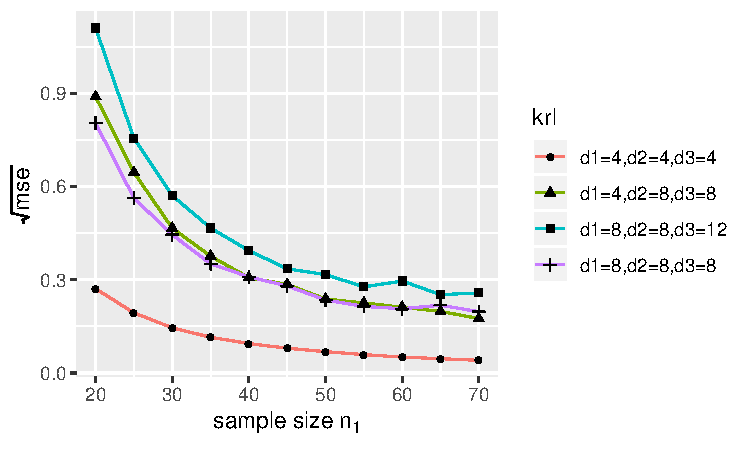
\includegraphics[scale=0.5]{figures/figure3/non-scale.pdf}}
	\subfloat[]{
\includegraphics[scale=0.5]{figures/figure3/rescale.pdf}}
	\caption{Plots of the root mean squared error (RMSE) verus sample size when using our tensor clustering algorithm. Each curve corresponds to a fixed $(d_1,d_2,d_3)$. (a): Plots of average RMSE over 50 simulations against $n_1$; (b): Plots of averge RMSE over 50 simulations against $\sqrt{n_2n_3/logd_1}$. }
	
	\label{fig3}
\end{figure}

In the second simulation, we generate 50 non-sparse tensors with the same noise, size and cluster numbers each time. We use our approach (Algorithm \ref{alg:B}) to do the clustering and the result is shown as Table \ref{t1}. In both data size: 40*40*40 and 40*40*80, the CER on all modes are 0 when the noise is 4. As the noise goes up, the CER is increased gradually. Furthermore, from the $d_1=3, d_2=5, d_3=4$ cases, we notice that the CER of mode $i$ seems to be smaller when the number of clusters in the $i$th mode is less. \par 

To evaluate the performance of our approach on selecting the number of clusters, we generate 50 non-sparse tensors with the same noise, size and cluster numbers in each case in Table \ref{t2} as the third simulation.  The reason why we only evaluate the performance of estimation on cluster numbers on non-sparse tensor is in sparse case, the reasonable cluster numbers may not be unique. As expected, we achieve 100\% accuracy when the noise is 4, again. The overall accuracy goes down as the noise increased. Additionally, we notice that the smaller $d_i$ is, the more accurate the estimated value is. There are two extremely low overall accuracy which appears when noise is 12 and the tensor size is 40*40*40. However, the accuracy is improved quickly as the tensor size is enlarged to 40*40*80. We found that not only the accuracy of mode 3 decreased after we add observations on mode 3, but also the accuracy of other two modes decreased a lot. The reason is the length of an observation in mode 1 and mode 2 is longer than before. Therefore, it is very important for us to get enough observations to guarantee the overall accuracy.\par

In the forth simulation, the true cluster numbers are not given, so we estimate them first and then use the estimated true cluster numbers to estimate the partition of clusters as well as underlying mean signals. We set the true cluster numbers to be $d_1=3, d_2=5, d_3=4$ specifically here, and the results are shown in Table \ref{t3}. By looking into each mode separately, as the sample size of that mode increased , the CER of that mode decreased without any exception.\par  
\begin{table}
	\centering
	\begin{tabular}{|c|c|c|c|c|c|c|}
		\hline
		$n_1$&$n_2$&$n_3$&noise&CER(mode 1)&CER(mode 2)&CER(mode3)\\ \hline
		40&40&40&4&$\mathbf{0(0)}$&$\mathbf{0(0)}$&$\mathbf{0(0)}$\\
		40&40&40&8&$\mathbf{0(0)}$&0.0136(0.0226)&0.0005(0.0036) \\
		40&40&40&12&0.0365(0.0789)&0.12(0.0878)&0.0802(0.1009)\\
		40&45&50&4&$\mathbf{0(0)}$&$\mathbf{0(0)}$&$\mathbf{0(0)}$\\
		40&45&50&8&$\mathbf{0(0)}$&0.0027(0.0121)&$\mathbf{0(0)}$\\
		40&45&50&12&0.0158(0.0489)&0.0641(0.0629)&0.0336(0.0647)\\
		\hline
	\end{tabular}
	\caption{The CERs over 50 simulated tensors ($d_1=3, d_2=5, d_3=4$) each time.}
	\label{t3}
\end{table}

In the fifth simulation, we generate the tensor in two different ways. The new way to generate data is using $\sum_{s=1}^{S}d_s\mathbf{u_s}\mathbf{v_s}^T$ after giving the $S$.  First we randomly choose $\mathbf{u_s}$ and $\mathbf{v_s}$ from normal distribution where $i=1,...,S$. Then we add noise which is also sampled from normal distribution with given standard deviation. We name the tensor generated in this way as tensor with multiplicative clusters. In this simulation, we would check whether our method is still robust on the tensors with multiplicative cluster. Meanwhile, we would compare the performance of our approach with CPD k-means (do k-means clustering after using CP decomposition on the data tensor) under different noise and different kinds of tensor. To be more specific, when the data a a tensor with multiplicative clusters we just use the true rank that we use to generate the data tensor to do the CP k-means. As for the parameter $d_1, d_2, d_3$ in k-means, we also use the true parameter. We apply the true $d_1, d_2, d_3$ in our method, too. When the data is a tensor with constant clusters, we still use true $d_1, d_2, d_3$ in both methods. But for CPD k-means, we use BIC to select the best $S$ according to the formula: $error+\frac{log(n_1n_2n_3)(n_1+n_2+n_3-2)S}{n_1n_2n_3}$.  Here we set  $n_1=50,n_2=50,n_3=50$ and $d_1=4,d_2=4,d_3=4$ in all the cases, and add noise 0,10,20 to generate the tensors. Additionally, as for tensor with constant clusters, I randomly select underlying signals between -3 and 3; as for tensors with multiplicative clusters, I randomly select the elements of $\mathbf{u_s}$ and $\mathbf{v_s}$ between -3 and 3. Thus the mean signal of tensor with multiplicative clusters would be bigger than that of tensors with constant clusters. Therefore, the same noise would have bigger effect on the tensor with constant clusters. Our result is shown in Figure \ref{fig4}. To our surprise, our approach is not only better at working on tensor with constant clusters, but also better at working on tensor with multiplicative clusters. Furthermore, our approach shows more robustness under different level of noise, too. \par 

\begin{figure}
	\centering
	\subfloat[]{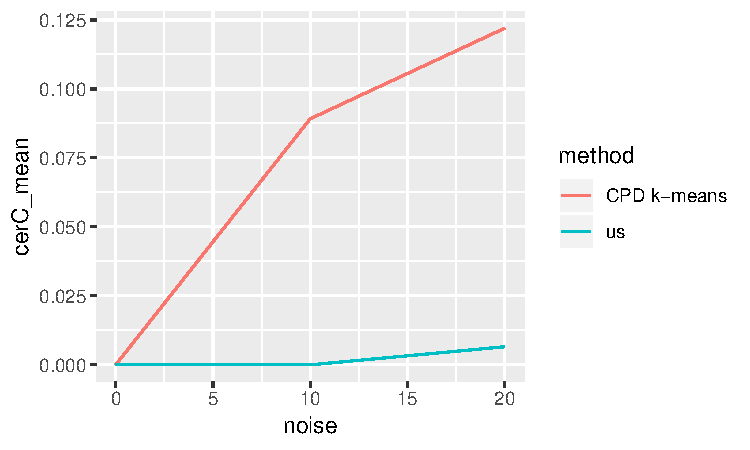
\includegraphics[scale=0.5]{figures/figure4/multidata.pdf}}
	\subfloat[]{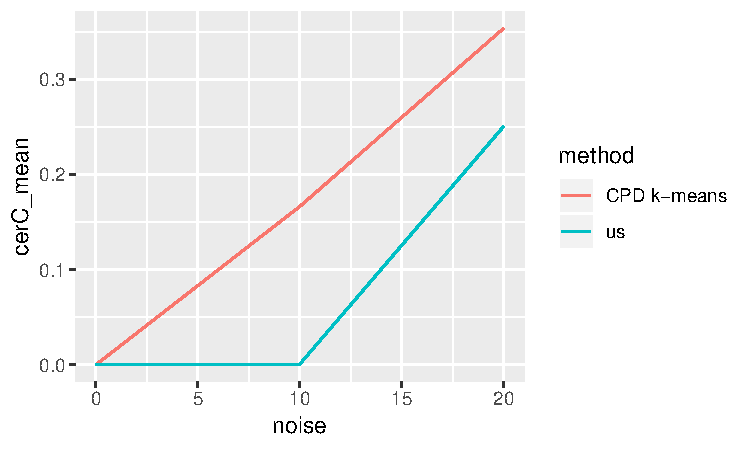
\includegraphics[scale=0.5]{figures/figure4/constantdata.pdf}}
	\caption{Plots of the mean CER C verus noise when using our tensor clustering algorithm and CPD k-means where $n_1=n_2=n_3=50, d_1=d_2=d_3=4$. Each curve corresponds to different method. (a): Plots of average CER in mode 1 over 50 simulations against noise while the  data is a tensor with multiplicative clusters where $S=3$; (b): Plots of averge CER in mode 1 over 50 simulations against noise while the data is a tensor with constant clusters.}
	\label{fig4}
\end{figure}



\textbf{Sparse case.} We also test the performance of our approach under different $\lambda$ when the data is sparse. The $\bar{\lambda}$ in Table \ref{t5} is the mean $\lambda$ we choose across 50 simulations on the same sparsity rate. According to Table \ref{t5}, the correct zero rate is increased with the increment on $\lambda$ while the correct one rate is exactly the opposite. As for the $\lambda$ we choose, it shows that the lowest total correct rate is 0.8586, which appears when noise is 8 and sparsity rate is 0.8. Overall, the $\lambda$ we select by BIC is fairly good, which does works better than other $\lambda$.

\section{Conclusion}
Sparsity is only one form of regularization. In specific applications, prior knowledge often suggests various constraints among parameters, which may be exploited to regularize parameter estimates. For example, in the stochastic block model, sometimes it may be reasonable to impose symmetry on the parameters along certain subsets of modes, which further reduces the dimension of the problem. In some other applications, non-negativity of parameter of parameter values may be enforced. In our software, we implement the common penalizations but leave .. .to further study. 



\bibliographystyle{unsrt}
\bibliography{tensor_wang}


\end{document}
